% ===== CHAPTER 1 =====
	\chapter{薛定谔方程}
	\section{量子化学}
	十七世纪末,艾萨克·牛顿(Isaac Newton)创立了\textbf{经典力学},即宏观物体的运动规律。二十世纪初,物理学家发现经典力学无法正确描述原子和分子的电子和原子核等极小粒子的行为。这类粒子的行为由一组称为\textbf{量子力学}的定律来描述。\\
	\indent \textbf{量子化学}将量子力学应用于化学问题。量子化学的影响在化学的各个分支中都很明显。物理化学家利用量子力学(借助统计力学)计算气体的热力学性质(如熵、热容量);解释分子光谱,从而通过实验确定分子性质(如分子几何形状、偶极矩、内旋转能垒、同分异构体之间的能量差异);从理论上计算分子性质;计算化学反应中过渡态的性质,从而估算速率常数;理解分子间作用力;以及处理固体中的成键问题。\\
	\indent 有机化学家利用量子力学估算分子的相对稳定性,计算反应中间产物的性质,研究化学反应的机理,以及分析和预测核磁共振谱。\\
	\indent 分析化学家广泛使用光谱法。只有利用量子力学,才能正确理解和解释光谱中的谱线频率和强度。\\
	\indent 无机化学家使用配体场理论(一种近似量子力学的方法)来预测和解释过渡金属络离子的性质。\\
	\indent 虽然重要生物分子的巨大尺寸使得对它们进行量子力学计算极其困难,但生物化学家们正开始从对生物分子构象、酶与底物结合以及生物分子溶解的量子力学研究中获益。\\
	\indent 量子力学决定了纳米材料(至少有一个维度在 1 nm到 100 nm之间的物体)的特性,目前正在开发处理纳米材料的计算方法。当材料的一个或多个尺寸小于 100 nm(尤其是小于 20 nm)时,其光学、电子、化学和其它特性就会发生与宏观材料显著不同的巨大变化。一个维度在 1 nm到 100 nm之间的半导体或金属物体称为\textit{量子阱};两个维度在此范围内的称为\textit{量子线};三个维度都在此范围内的称为\textit{量子点}。这些名称中的 “量子 ”一词表明量子力学在决定此类材料特性方面发挥了关键作用。许多人猜测,纳米科学和纳米技术将带来 “下一次工业革命”。\\
	\indent 计算机计算速度的迅速提高和分子计算新方法(如密度泛函理论-参见第 16.4 节)的发展,使量子化学成为化学各个领域的实用工具。现在,有几家公司出售用于分子量子化学计算的量子化学软件。这些软件不仅适用于量子化学家,也适用于其他各类化学家。由于量子化学及相关理论和计算方法的作用日益显著,美国化学学会于 2005 年开始出版新的期刊《化学理论与计算杂志》(Journal of Chemical Theory and Computation)。\\
	\indent “\textit{量子力学......几乎是所有现代科学技术的基础。它支配着晶体管和集成电路的行为......并且是......现代化学和生物学的基础。}”[斯蒂芬·霍金(Stephen Hawking),《时间简史》,1988 年,Bantam 出版社,第 4 章)]
	
	\section{量子力学的历史背景}
	\noindent 量子力学的发展起源于 1900 年普朗克(Planck)对加热固体发出的光的研究,因此我们首先要讨论光的本质。\\
	\indent 1803 年,托马斯·杨(Thomas Young)通过观察光穿过两个相邻针孔时的衍射和干涉,为光的波动性提供了令人信服的证据。(\textit{衍射}是波绕障碍物弯曲。\textit{干涉}是将两个频率相同的波结合在一起,产生一个波,该波在空间每一点的扰动是每个干涉波在该点产生的扰动的代数和或矢量和。参见任何一年级物理课本)。\\
	\indent 1864 年,詹姆斯·克拉克·麦克斯韦(James Clerk Maxwell)建立了四个方程,即麦克斯韦方程组(Maxwell's equations),统一了电学和磁学定律。麦克斯韦方程预言:加速的电荷会以电磁波的形式辐射能量,电磁波由振荡的电场和磁场组成。麦克斯韦方程预测的这些波的速度与实验测得的光速相同。\\
	\indent 1888 年,海因里希·赫兹(Heinrich Hertz)根据麦克斯韦方程组的预测,探测到了电火花中加速电荷产生的无线电波。这使物理学家确信,光确实是一种电磁波。\\
	\indent 所有电磁波在真空中都以$c = 2.998 \times 10^8$ m/s的速度传播。电磁波的频率$\nu$和波长$\lambda$的关系是
	\begin{equation}
		\boxed{\lambda \nu = c}
		\label{eq:1.1 wavelength and frequency}
	\end{equation}
	(方框内的等式应牢记;附录中给出了希腊字母表)。根据电磁波的频率,人们给电磁波进行了分类。按照频率递增的顺序依次为无线电波、微波、红外线辐射、可见光、紫外线辐射、X 射线和$\gamma$射线。我们用光来表示任何一种电磁辐射。可见光和紫外线辐射的波长以前用埃(\AA)来表示,现在用纳米(nm)来表示:
	\begin{equation}
		\boxed{1 \: \text{nm} = 10^{-9} \: \text{nm}, \qquad 1 \: \text{\AA}= 10^{-10} \: \text{m} = 0.1 \: \text{nm}}
		\label{units:1.2 nm and angstroms}
	\end{equation}
	\indent 19 世纪 90 年代,物理学家测量了在固定温度下加热黑体发出的各种频率的光强度,并在多个温度下进行了这些测量。\textit{黑体}是一种能吸收落在其上的所有光线的物体。一种对黑体对良好近似是一个带有小孔的空腔。1896 年,物理学家维恩(Wien)提出了黑体辐射与光频和黑体温度的关系式:$I=a\nu^3/\text{e}^{b\nu /T}$,其中$a$与$b$是经验常数,$I \text{d} \nu$是黑体在单位时间和单位表面积内辐射的频率在$\nu$到$\nu + \text{d} \nu$范围内的能量,其中$\text{d} \nu$是一个无穷小的频率范围。维恩的公式很好地拟合了 1896 年的黑体辐射数据,但他对该公式的理论论证却不令人满意。\\
	\indent 1899-1900 年,对黑体辐射的测量扩展到了比以前更低的频率,维恩公式在低频下显示出较大的偏差。这些偏差促使物理学家马克斯·普朗克(Max Planck)于 1900 年 10 月提出了以下公式$I=a \nu^3 / \left(\text{e}^{b\nu / T}-1\right)$,并发现该公式适用于所有频率的数据。\\
	\indent 提出这个公式后,普朗克一直在寻找理论依据。1900 年 12 月,他向德国物理学会提交了他的公式的理论推导。普朗克假定黑体中的辐射发射器和吸收器是与空腔中的电磁辐射处于平衡状态的谐振电荷(“谐振子”)。他假设频率为$\nu$的谐振子的总能量由$N$个不可分割的 “能量元素”组成,每个能量元素的大小为$h\nu$,其中$N$为整数,$h$(普朗克常数)是物理学中的一个新常数。普朗克将这些能量元素分布在谐振子中。实际上,每个谐振子的能量必须是$h\nu$的整数倍(尽管普朗克没有明说)。因此,每个谐振子的能量都被量子化了,这意味着谐振子的能量只允许是某些分立的值。普朗克的理论导出了$a=2 \pi  h/c^2$和$b=h/k$,其中$k$是玻尔兹曼(Bolzmann)常量。通过拟合实验中得到的黑体辐射曲线,普朗克常数为$h=6.6 \times 10^{-34}$ J$\cdot$s。\\
	\indent 普朗克的工作通常被认为是量子力学的开端。然而,物理学史学家们一直在争论:1900 年的普朗克究竟是将能量量子化视为对物理现实的描述,还是仅仅将其视为一种数学近似,从而使他能够获得正确的黑体辐射公式。[见 O. Darrigol,Centaurus,43,219 (2001);C. A. Gearhart,Phys. Perspect.,4,170 (2002)(可在线查阅:employees.csbsju.edu/cgearhart/Planck/PQH.pdf;S. G. Brush,Am. J.Phys., 70, 119 (2002) (www.punsterproductions.com/~sciencehistory/cautious.htm).]。物理历史学家克拉格(Kragh)指出:“\textit{如果说 1900 年 12 月物理学发生了一场革命,似乎没有人注意到它。普朗克也不例外,赋予他的工作的重要性在很大程度上是一种历史重构。}”(H. Kragh,《物理学世界》,2000 年 12 月,第 31 页)\\
	\indent 能量量子化的概念与以往物理学的所有理念直接相悖。经典力学认为:物质体的能量可以连续变化。然而,只有在能量量子化的假设下,才能得到正确的黑体辐射曲线。\\
	\indent 能量量子化的第二个应用是\textit{光电效应}。在光电效应中,光照射到金属上会导致电子被激发。波的能量与其强度成正比,而与其频率无关。因此光的电磁波图象会让人想到:发射的光电子的动能会随着光强度的增加而增加,但不会随着光频率的变化而变化。\\
	\indent 1905 年,爱因斯坦(Einstein)指出:将光视为由粒子状实体(称为\textit{光子})组成的集合体,每个光子都具有能量
	\begin{equation}
		\boxed{E=h\nu}
		\label{eq:1.3 photoelectric effect equation}
	\end{equation}
	就可以解释这些观测结果。当金属中的电子吸收光子时,所吸收的光子能量的一部分被用来克服将电子固定在金属中的力,剩余的能量则转化为电子逸出后的动能。由能量守恒,有$h\nu = \phi+ T$,其中$\phi$是电子逸出金属表面所需的最小能量(金属的功函数),$T$是被激发电子的最大动能。提高光的频率$\nu$会增加光子能量,从而增加被激发电子的动能。增加固定频率下的光强度会增加光子撞击金属的速度,从而增加电子的发射速度,但不会改变每个发射电子的动能。(克拉格认为:“\textit{可以有力地证明,是爱因斯坦首先认识到了量子理论的本质。}”;H. Kragh,《物理世界》,2000 年 12 月,第 31 页)\\
	\indent 光电效应表明:除了在衍射实验中表现出波动性外,光还可以表现出粒子性。\\
	\indent 1907 年,爱因斯坦将能量量子化应用于固体元素中原子的振动。假设每个原子在每个方向$\left(x,y,z\right)$上的振动能量被限制为$h\nu_{vib}$的整数倍,其中振动频率$\nu_{vib}$是元素的性质。爱因斯坦利用统计力学推导出固体恒容热容$C_V$的表达式。他的公式与已知的钻石$C_V$与温度的关系数据相当吻合。\\
	\indent 现在我们来考虑物质的结构。\\
	\indent 19 世纪末,对放电管和自然放射性的研究表明:原子和分子是由带电粒子组成的。电子带有负电荷,而质子带有与电子电荷大小相等但符号相反的正电荷,其质量是电子的 1836 倍。原子的第三种成分-中子(1932 年发现)不带电荷,比质子稍重。\\
	\indent 从 1909 年开始,卢瑟福(Rutherford)、盖革(Geige)和马斯登(Marsden)反复将一束$\alpha$粒子穿过薄金属箔,并让它们落在荧光屏上,从而观察到粒子的偏转。$\alpha$粒子是从天然放射性衰变中获得的带正电荷的氦核。大多数$\alpha$粒子通过金属箔时基本上没有发生偏转,但令人惊讶的是,少数粒子发生了很大的偏转,有些粒子向后偏转。如果正电荷遍布整个原子[正如 J. J. 汤姆逊(Thomson)在 1904 年提出的那样],那么一旦高能$\alpha$粒子穿透原子,斥力就会减弱,根据经典静力学,在原子中心的斥力为零。因此,卢瑟福得出结论:只有当正电荷集中在一个微小而沉重的原子核中时,才会发生如此大的偏转。\\
	\indent 原子包含一个极小(半径为$10^{-13}$到$10^{-12}$ cm)的重核,由中子和$Z$个质子组成,其中$Z$是原子序数,原子核外有$Z$个电子,带电粒子的相互作用遵循库仑定律。(核子在原子核内通过强相互作用结合在一起,这与我们无关)原子的半径约为1 \AA,气体动力学理论的结果就表明了这一点。\\
	\indent 原子和分子的化学性质是由其电子结构决定的,因此就产生了电子运动和能量的性质问题。由于原子核的质量远大于电子,我们认为原子核的运动与电子的运动相比是微小的。\\
	\indent 1911 年,卢瑟福提出了原子的行星模型,其中电子以不同的轨道围绕原子核旋转,就像行星围绕太阳旋转一样。然而,这一模型存在一个根本性的难题。根据经典电磁理论,加速的带电粒子会以电磁波(光波)的形式辐射能量。以恒定速度围绕原子核旋转的电子正在被加速,因为其速度矢量的方向在不断变化。因此,卢瑟福模型中的电子应该不断地通过辐射损失能量,从而向原子核螺旋运动。因此,根据经典(19 世纪)的物理学,卢瑟福的原子结构是不稳定的,会发生坍缩。\\
	\indent 1913 年,尼尔斯·玻尔(Niels Bohr)将能量量子化的概念应用于氢原子,提出了解决这一难题的可行方法。玻尔假定氢原子中电子的能量是量子化的,电子只能在一系列允许的轨道中的一个轨道上运动。当电子从一个玻尔轨道过渡到另一个玻尔轨道时,一个频率$\nu$满足
	\begin{equation}
		\boxed{E_{upper}-E_{lower}=h\nu}
		\label{eq:1.4 Higher state to lower state delta energy}
	\end{equation}
	的光子被吸收或激发。其中$E_{upper}$和$E_{lower}$是高低两个状态的能量(能量守恒)。玻尔假定电子从自由(电离)态过渡到束缚轨道时会发射出一个光子,其频率是电子在束缚轨道中经典旋转频率的二分之一的整数倍,他利用经典力学推导出了氢原子能级的计算公式。利用(\ref{eq:1.4 Higher state to lower state delta energy}),他得到了与观测到的氢谱一致的结果。然而,用玻尔理论拟合氦光谱的尝试却失败了。此外,该理论无法解释分子中的化学键。\\
	\indent 玻尔模型的失败源于使用经典力学来描述原子中的电子运动。原子光谱显示出离散的频率,这表明只有某些能量的运动是允许的;以及电子能量是量子化的。然而,经典力学允许连续的能量范围。因此,路易斯·德布罗意(Louis de Broglie)在 1923 年提出:电子的运动可能具有波的一面。质量为$m$、速度为$v$的电子将具有波长
	\begin{equation}
		\lambda=\frac{h}{mv}=\frac{h}{p}
		\label{eq:1.5 de Brogile equation}
	\end{equation}
	其中$p$是线性动量。德布罗意通过与光子的类比推理得出公式(\ref{eq:1.5 de Brogile equation})。根据爱因斯坦的狭义相对论,光子的能量可以用$E=pc$表示,其中$c$是光速,$p$是光子的动量。利用$E_{photon}=h\nu$可以得到光子以$c$的速度运动时的$pc=h\nu =hc/\lambda$和$\lambda = h/p$。方程式 (\ref{eq:1.5 de Brogile equation}) 是电子相应的方程式。\\
	\indent 1927 年,戴维森(Davisson)和格尔默(Germer)通过实验证实了德布罗意的假设,他们从金属中反射电子并观察到衍射效应。1932 年,斯特恩(Stern)在氦原子和氢分子中观察到了同样的效应,从而验证了波效应并非电子所特有,而是微观粒子运动的某种普遍规律的结果。通过衍射光栅可以观察到大至 C$_{48}$H$_{26}$F$_{24}$N$_8$O$_8$的分子的衍射和干涉现象	。[T. Juffmann 等,Nat. Nanotechnol.,7,297 (2012)]。有关分子干涉图案形成的影片,请访问 www.youtube.com/watch?v=vCiOMQIRU7I。\\
	\indent 因此,电子的行为在某些方面像粒子,而在另一些方面则像波。我们面临着物质(以及光)表面上自相矛盾的 “波粒二象性”。电子怎么可能既是粒子(局部实体),又是波(非局部实体)呢?答案是电子既不是波也不是粒子,而是另一种东西。用经典物理学的波或粒子概念来准确描述电子的行为是不可能的。经典物理学的概念是根据宏观世界的经验发展而来的,并不能正确描述微观世界。进化塑造了人类大脑,使其能够理解并有效处理宏观现象。人类神经系统的发展并不是为了处理原子和分子层面的现象,因此我们无法完全理解这些现象也就不足为奇了。\\
	\indent 虽然光子和电子都表现出明显的二元性,但它们并不是同一类实体。光子在真空中以$c$的速度运动,其静止质量为零;而电子始终具有$v<c$和非零静止质量。光子必须始终按相对论处理,但速度远小于$c$的电子可以按非相对论处理。
	
	\section{不确定性关系}
	让我们来看看波粒二象性对同时测量微观粒子的$x$坐标和线动量$x$分量的尝试有什么影响。我们从一束动量为$p$、沿$y$方向运动的粒子束开始,让粒子束落在一个窄缝上。狭缝后面是一块照相板。见图\ref{fig:1.1}。\\
	\indent 粒子通过宽度为$w$的狭缝时,其$x$坐标的不确定性为$w$。我们将这种$x$值的分布称为$\Delta x$,即有$\Delta x = w$。\\
	\indent 由于微观粒子具有波的特性,它们会被狭缝衍射,在平板上产生衍射图样(就像光束一样)。图 \ref{fig:1.1}中图形的高度表示到达给定点的粒子数量。衍射图样显示:当粒子被狭缝衍射时,它们的运动方向发生了改变,因此部分动量被转移到了$x$方向。动量在$x$方向上的分量$p_x$等于动量矢量$\overrightarrow{p}$在$x$方向上的投影。向上偏转$\alpha$角的粒子的动量满足$p_x=p\sin \alpha$;向下偏转$\alpha$角的粒子的动量满足$p_x=-p \sin \alpha$。由于大多数粒子的偏转范围在$-\alpha$到$\alpha$之间,其中$\alpha$是与衍射图样中第一个最小值的夹角,因此我们将以中心衍射峰中动量值的一般作为动量$x$分量不确定性$\Delta p_x$的量度:$\Delta p_x = p \sin \alpha$。\\
	\indent 因此,在狭缝处进行测量,有
	\begin{equation}
		\Delta x \Delta p_x = pw \sin \alpha 
		\label{eq:1.6 diffract equation on x}
	\end{equation}
	
	\begin{figure}[h!]
		\centering
		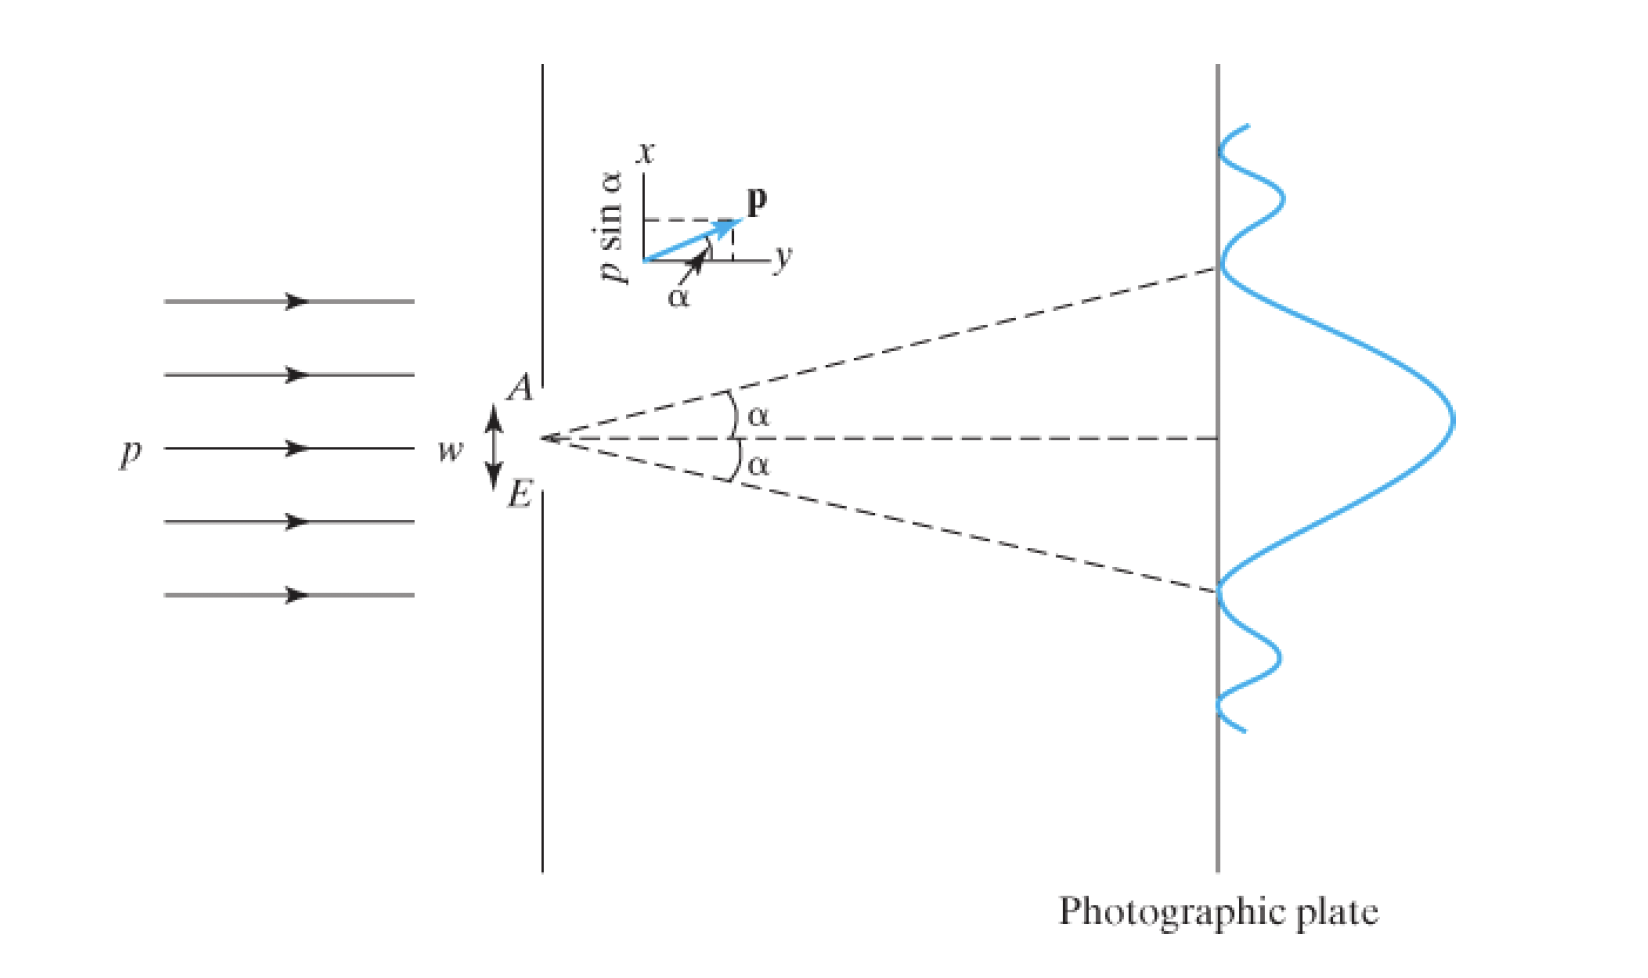
\includegraphics[width=0.8\textwidth]{/users/administrator/desktop/repo/quantumchemistry/Figures/1.1.png}  % 图片路径
		\caption{\text{狭缝的电子衍射}}
		\label{fig:1.1}
	\end{figure}
	\begin{figure}[h!]
		\centering
		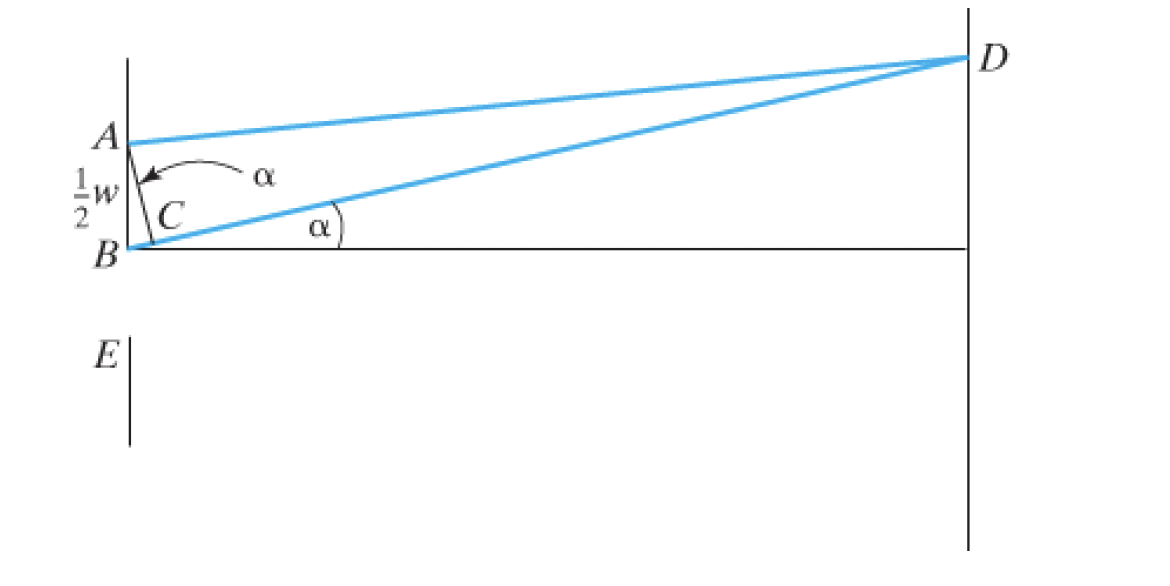
\includegraphics[width=0.6\textwidth]{/users/administrator/desktop/repo/quantumchemistry/Figures/1.2.png}
		\caption{\text{计算一级衍射的最小值}}
		\label{fig:1.2}
	\end{figure}
	
	\indent 第一个衍射最小值出现的角度$\alpha$很容易计算。出现第一个最小值的条件是:通过狭缝上边缘的粒子和通过狭缝中心的粒子所经过的距离之差应等于$\frac{1}{2}\lambda$,其中$\lambda$是相关波的波长。这样,从狭缝顶部发出的波与从狭缝中心发出的波正好相位相反,它们相互抵消。从狭缝中点以下距离$d$处发出的波与从狭缝顶部以下距离$d$处发出的波相互抵消。在图 \ref{fig:1.2}中画出$AC$,使 $AD=CD$,则路径长度之差为$BC$。狭缝到屏幕的距离比狭缝宽度大。因此,由于$AD$和$BD$几乎平行,则$\angle ACB$基本上是直角,因此$\angle BAC = \alpha$ ,路径差$BC$就是$\frac{1}{2}w \sin \alpha$。 设$BC$等于$\frac{1}{2}\lambda$,我们就得到了$w\sin\alpha=\lambda$,公式(\ref{eq:1.6 diffract equation on x}) 就变成了$\Delta x \Delta p_x=p\lambda$,其中波长$\lambda$由德布罗意关系式$\lambda=h/p$给出,因此$\Delta x \Delta p_x=h$。由于不确定度尚未精确定义,因此使用等号并不合适。我们可以用 
	\begin{equation}
		\Delta x \Delta p_x \approx h
		\label{eq:1.7 uncertinty on x}
	\end{equation}
	来表示$x$方向上的不确定性,同时$p_x$具有与普朗克常数相当的的数量级。\\
	\indent 尽管我们只在一种实验装置上证明了(\ref{eq:1.7 uncertinty on x}),但其有效性是普遍的。无论如何尝试,微观 “粒子 ”的波粒二象性都限制了我们同时测量这种粒子的位置和动量的能力。我们对位置的测定越精确,对动量的测定就越不准确。(在图\ref{fig:1.1}中,$\sin \alpha = \lambda / w$,因此缩小狭缝会增加衍射图样的扩散)这种限制就是沃纳·海森堡(Werner Heisenberg)于 1927 年发现的\textbf{不确定性关系}。\\
	\indent 由于波粒二象性,测量行为会给被测系统带来不可控制的干扰。我们从粒子具有精确的$p_x$值(零)开始。通过施加狭缝,我们测量了粒子的$x$坐标,精确度为$w$,但这次测量给粒子的$p_x$值带来了不确定性。测量改变了系统的状态。
	
	
	\section{含时薛定谔方程}
	经典力学只适用于宏观粒子。对于微观 “粒子”,我们需要一种新的力学形式,即\textbf{量子力学}。为简单起见,我们将讨论一个单粒子的一维系统。\\
	\indent 在经典力学中,粒子的运动遵循牛顿第二定律:
	\begin{equation}
		\boxed{F = ma = m \frac{\text{d}^2x}{\text{d}t^2}}
		\label{eq:1.8 Newton's second law}
	\end{equation}
	其中$F$是作用在粒子上的合外力,$m$是粒子的质量,$t$是时间;$a$是加速度,由$a = \text{d} v / \text{d}t = \left(\text{d} / \text{d}t\right)\left(\text{d}x / \text{d}t\right) = \text{d}^2x / \text{d} t^2$给出,其中$v$是速度。方程(\ref{eq:1.8 Newton's second law})包含坐标$x$对时间的二阶导数。为了求解这个方程,我们必须进行两次积分。这就引入了两个积分常量$c_1$和$c_2$,有
	\begin{equation}
		x=g\left(t,c_1,c_2\right)
		\label{eq:1.9 function of the x-coordinate}
	\end{equation}
	其中$g$是时间的某个函数。我们现在要问:在某一特定时间$t_0$,我们必须掌握哪些信息才能预测粒子未来的运动?如果我们知道在$t_0$时刻,粒子位于$x_0$处,则有
	\begin{equation}
		x_0=g\left(t_0,c_1,c_2\right)
		\label{eq:1.10 initial function of the x-coordinate}
	\end{equation}
	由于我们需要确定两个常数,因此需要更多信息。将(\ref{eq:1.9 function of the x-coordinate})左右两边对时间求导,有
	\begin{equation*}
		\frac{\text{d} x }{\text{d}t} = v = \frac{\text{d}}{\text{d} t} g\left(t,c_1,c_2\right)
		\label{eq*:derivative of g function with respect to time}
	\end{equation*}
	如果我们也知道在$t_0$时刻,粒子具有速度$v_0$,那么有进一步的关系
	\begin{equation}
		v_0 = \eval{\frac{\mathrm{d}}{\mathrm{d} t} g(t, c_1, c_2)}_{t = t_0}
		\label{eq:1.11 v_0's equation}
	\end{equation}
	知道$x_0$和$v_0$后,我们可以用方程(\ref{eq:1.10 initial function of the x-coordinate})和(\ref{eq:1.11 v_0's equation})求出$c_1$和$c_2$。知道$c_1$和$c_2$后,就可以用方程(\ref{eq:1.9 function of the x-coordinate})来精确预测粒子在未来的运动。\\
	 \indent 作为式(\ref{eq:1.8 Newton's second law})至(\ref{eq:1.11 v_0's equation})的例子,考虑一个粒子在地球重力场中的运动。取垂直向上为$x$轴正方向,则作用在粒子上的合外力方向垂直向下,大小为$-mg$,其中$g$是重力加速度。则牛顿第二定律(\ref{eq:1.8 Newton's second law})形式为$-mg=m\mathrm{d}^2x/\mathrm{d}t^2$,所以$\mathrm{d}^2x/\mathrm{d}t^2=-g$。积分一次,有$\mathrm{d}x/\mathrm{d}t=-gt+c_1$。如果我们知道粒子在$t_0$时刻的速度为$v_0$,就可以求出积分常量$c_1$。又由于$v=\mathrm{d}x/\mathrm{d}t$,将$v_0=-gt_0+c_1$即$c_1=v_0+gt_0$带入,有$\mathrm{d}x/\mathrm{d}t=-gt+gt_0+v_0$。再次积分,我们引入了另一个积分常量$c_2$。如果我们知道粒子在$t_0$时刻的位置为$x_0$,则可以求出$c_2$。	因此,我们有$x=x_0-\frac{1}{2}g\left(t-t_0\right)^2+v_0\left(t-t_0\right)$。知道了在$t_0$时刻粒子的$x_0$和$v_0$,我们就能预测粒子未来的运动轨迹。\\
	 \indent 在一维范围内运动的粒子的经典力学势能$V$的定义为满足
	 \begin{equation}
	 	\boxed{\frac{\partial V \left(x,t\right)}{\partial x} = -F\left(x,t\right)}
	 	\label{eq:1.12 Potential energy in classical mechanics}
	 \end{equation}
	 例如,对于一个在地球重力场中运动的粒子,有$\partial V / \partial x = -F = mg$,积分一次,有$V = mgx+c$,其中$c$为积分常量。我们可以任意选择我们想要的零势能面。令$c=0$,我们有势能函数$V=mgx$。\\
	 \indent 经典力学中的 “\textbf{状态} ”一词是指系统中每个粒子在某一时刻的位置和速度,以及作用在粒子上的力。根据牛顿第二定律,给定一个系统在任何时候的状态,它的未来状态和未来运动都是完全确定的,如式(\ref{eq:1.9 function of the x-coordinate})-(\ref{eq:1.11 v_0's equation})所示。牛顿定律在解释行星运动方面取得的巨大成功让许多哲学家将牛顿定律作为哲学决定论的论据。数学家和天文学家拉普拉斯(Laplace)(1749-1827)假定宇宙是由服从牛顿定律的粒子组成的。因此,给定宇宙在某一时刻的状态,宇宙万物未来的运动是完全确定的。原则上,一个能知道宇宙任何瞬间状态的超级星体可以计算出所有未来的运动。
	% 小字号且缩进的段落
	\begin{quote}
		\small % 字号小一号(可选 \footnotesize 更小)
		\noindent % 取消首行缩进(可选)
		尽管经典力学是确定性的,但许多经典力学系统(例如,在重力、摩擦力和周期性变化的驱动力影响下摆动的摆)在系统参数的一定范围内表现出混沌行为。在混沌系统中,运动对粒子位置和速度的初始值以及作用力异常敏感,两个初始状态相差一个实验无法检测的量,最终会导致系统的未来行为大相径庭。因此,由于测量初始状态的精度有限,即使系统服从确定性方程,实际上也不可能预测混沌经典力学系统的长期行为。对太阳系行星数千万年轨道的计算机计算表明,行星的运动是混沌的。[I. Peterson, 《牛顿的钟:混沌的太阳系》,Freeman,1993 年;J. J. Lissauer,Rev. Mod. 71, 835 (1999)]
	\end{quote}
	\indent 
	\indent 只要精确了解经典力学系统的当前状态,我们就能预测其未来状态。然而,海森堡不确定性原理表明:我们无法同时确定微观粒子的精确位置和速度,因此无法获得经典力学所需的数据来预测系统的未来运动。 在量子力学中,我们必须满足于对未来精确运动的不完全预测。\\
	\indent 我们研究量子力学的方法是\textit{假设}基本原理,然后利用这些假设推导出实验可检验的结果,例如原子的能级。为了描述量子力学中一个系统的\textbf{状态},我们假设存在一个粒子坐标的函数$\Psi$,称为\textbf{状态函数}或\textbf{波 函数}(通常写作\textbf{波函数})。由于状态一般会随时间变化,因此$\Psi$也是时间的函数。对于一个单粒子的一维系统,我们有$\Psi=\Psi\left(x,t\right)$。波函数包含了一个系统所有可能的信息,因此我们不说 “波函数$\Psi$所描述的状态”,而只说 “状态$\Psi$”。 牛顿第二定律告诉我们:如何通过对经典力学系统当前状态的了解来找到它的未来状态。而要根据量子力学系统当前的状态找到它未来的状态,我们需要一个方程来告诉我们波函数是如何随时间变化的。对于单粒子的一维系统,将这个方程假定为
	\begin{equation}
		-\frac{\hbar}{\mathrm{i}}\frac{\partial \Psi \left(x,t\right)}{\partial t}= -\frac{\hbar^2}{2m}\frac{\partial^2 \Psi \left(x,t\right)}{\partial x^2}+ V\left(x,t\right)\Psi\left(x,t\right)
		\label{eq:1.13 Time-dependent Schödinger equation}
	\end{equation}
	其中常数$\hbar$(约化普朗克常数)定义为
	\begin{equation}
		\boxed{\hbar \equiv \frac{h}{2 \pi}}
		\label{eq:1.14 h-bar's definition}
	\end{equation}
	\indent 1926 年,奥地利物理学家埃尔温·薛定谔(Erwin Schrödinger)(1887-1961)建立了波函数的概念及其随时间变化的方程。这个被称为\textbf{含时薛定谔方程}(或\textbf{薛定谔波方程})中,$\mathrm{i}$是虚数单位,$m$是粒子的质量,$V\left(x,t\right)$是系统的势能函数。(量子力学中许多具有重要历史意义的论文可在 dieumsnh.qfb.umich.mx/archivoshistoricosmq 网站上查阅)\\
	\indent 含时薛定谔方程包含波函数对时间的一阶导数,如果我们知道$t_0$时刻的波函数,就可以计算出未来任意时刻的波函数(状态)。\\
	\indent 波函数包含了我们可能知道的关于它所描述的系统的所有信息。关于粒子$x$坐标的测量结果,$\Psi$给了我们什么信息?我们不能指望$\Psi$会像经典力学系统的状态那样具有涉及位置的明确说明。这个问题的正确答案是在薛定谔发现薛定谔方程后不久,由马克斯·玻恩(Max Born)给出的。玻恩推测:对于单粒子的一维系统,
	\begin{equation}
		\left|\Psi \left(x,t\right)\right|^2 \mathrm{d}x
		\label{exp:1.15 probability of a particle}
	\end{equation}
	给出了在$t$时刻,在$x$到$x+ \mathrm{d}x$范围内找到该粒子的概率。在(\ref{exp:1.15 probability of a particle})中,两条竖线表示绝对值,$\mathrm{d}x$表示$x$轴上一个无限小的长度。函数$\left|\Psi \left(x,t\right)\right|^2$是在$x$轴上不同位置找到粒子的\textbf{概率密度}。(第 1.6 节回顾了概率)例如,假设在某个特定时间$t_0$,粒子处于由波函数$a^2\mathrm{e}^{-2bx^2}$描述的特征状态,其中$a$和$b$是实常数。如果我们在$t_0$时刻观测该粒子的位置,会得到任意的$x$值,因为概率密度$a^2\mathrm{e}^{-2bx^2}$处处非零。由于$\left|\Psi\right|^2$在原点取到最大值,因此在$x=0$附近的$x$值比其他地方的更有可能被取到。\\
	\indent 为了将$\Psi$与实验测量联系起来,我们需要许多完全相同的非相互作用系统,每个系统都处于相同的状态$\Psi$。如果我们对$n$个系统进行了$n$次测量,令$\mathrm{d}n_x$表示在$x$和$x+\mathrm{d}x$之间找到粒子的测量次数,那么$\mathrm{d}n_x/n$就是在$x$和$x+\mathrm{d}x$之间找到粒子的概率。因此,有
	\begin{equation*}
		\frac{\mathrm{d}n_x}{n} = \left|\Psi\right|^2\mathrm{d}x
	\end{equation*}
	而$\left(1/n\right) \mathrm{d}n_x / \mathrm{d}x$与$x$的关系图则给出了概率密度$\left|\Psi\right|^2$与$x$的函数关系。也许有人认为,我们可以通过一个处于$\Psi$状态的系统,反复测量粒子的位置来找到概率密度函数。这种方法是错误的,因为测量过程通常会改变系统的状态。我们在讨论不确定性原理(第 1.3 节)时看到过一个这方面的例子。\\
	\indent 量子力学是\textit{统计性质}的。在知道状态的情况下,我们无法准确预测位置测量的结果;我们只能预测各种可能结果的\textit{概率}。氢原子的玻尔理论规定了电子的精确路径,因此不是正确的量子力学图景。\\
	\indent 量子力学并没有说电子像波一样分布在空间的很大区域。相反,用于描述电子运动的概率模式(波函数)表现得像波,并满足波方程。\\
	\indent 波函数如何为我们提供位置以外的其他属性信息,将在后面的章节中讨论。\\
	\indent 热力学公设(热力学第一、第二和第三定律)是由宏观经验提出的,因此相当容易理解。量子力学的公设是从微观世界的角度阐述的,显得相当抽象。不要指望第一次接触就能完全理解量子力学公设。随着我们对各种实例的处理,对这些公设的理解会加深。\\
	\indent 我们引入了薛定谔方程,却没有试图证明它的合理性,这可能会让读者感到困惑。通过几何光学和经典力学之间的类比,以及波光学和量子力学之间的类比,我们可以证明薛定谔方程的合理性。几何光学是波光学的近似,在光的波长远小于仪器尺寸时有效。(同样,经典力学是波动力学的近似,当粒子的波长远小于仪器的尺寸时有效。我们可以根据已知的几何光学方程和波光学方程之间的关系,猜测如何从经典力学中得到量子力学的正确方程。由于许多化学家对光学并不特别熟悉,因此省略了这些论证。无论如何,这些类比只能使薛定谔方程看起来\textit{可信}。它们不能用来\textit{推导}或\textit{证明}这个方程。薛定谔方程是理论的一个\textit{假设},要通过其预测与实验的一致性来检验。(关于薛定谔得出方程的推理细节,请参阅 Jammer,第 5.3 节。参考文献中的作者姓名用斜体标出)\\
	\indent 量子力学为微观粒子提供了运动规律。从实验上看,宏观物体遵从经典力学。因此,要使量子力学成为有效的理论,当我们从微观粒子过渡到宏观粒子时,量子力学应还原为经典力学。量子效应与德布罗意波长$\lambda=h/mv$有关。由于$h$非常小,宏观物体的德布罗意波长近似为零。因此,在极限$\lambda \rightarrow 0$中,我们期望含时薛定谔方程能够还原为牛顿第二定律。我们可以证明这一点(见问题 7.59)。\\
	\indent 狭义相对论与经典力学的关系也存在类似的情况。在以$c$为光速的极限$v/c \rightarrow 0$中,狭义相对论可还原为经典力学。我们将要发展的量子力学形式将是非相对论的。相对论与量子力学的完全融合尚未实现。\\
	\indent 从历史上看,量子力学是由海森堡、玻恩和乔丹(Jordan)于 1925 年首次使用矩阵提出的,比薛定谔于 1926 年使用微分方程提出的量子力学早几个月。薛定谔证明:海森堡公式(称为\textbf{矩阵力学})等同于薛定谔公式(称为\textbf{波动力学})。1926 年,狄拉克和乔丹分别独立地用一种称为\textit{变换理论}的抽象版本提出了量子力学,它是矩阵力学和波动力学的概括(见《狄拉克》)。1948 年,费曼设计出了量子力学的\textit{路径积分}公式 [R. P. Feynman, Rev. Mod. Phys., 20, 367 (1948); R. P. Feynman,Rev. Mod. Phys., 20, 367(1948); R. P. Feynman and A. R. Hibbs, Quantum Mechanics and Path Integrals, McGraw-Hill, 1965]。
	
	\section{定态薛定谔方程}
	含时薛定谔方程(\ref{eq:1.13 Time-dependent Schödinger equation}) 看上去很可怕。幸运的是,量子力学在化学中的许多应用都不使用这个方程。取而代之的是更简单的定态薛定谔方程。现在,我们从一维单粒子的含时薛定谔方程导出定态薛定谔方程。\\
	\indent 首先,我们只讨论一种特殊情况,即势能$V$不是时间的函数,而只取决于$x$。系统没有受到与时间相关的外力作用会导致此情况。此时,含时薛定谔方程为
	\begin{equation}
		-\frac{\hbar}{\mathrm{i}}\frac{\partial \Psi \left(x,t\right)}{\partial t}= -\frac{\hbar^2}{2m}\frac{\partial^2 \Psi \left(x,t\right)}{\partial x^2}+ V\left(x,t\right)\Psi\left(x,t\right)
		\label{eq:1.16 Time-dependent Schödinger equation}
	\end{equation}
	将式(\ref{eq:1.16 Time-dependent Schödinger equation})的解假设为时间函数和坐标$x$函数的乘积:
	\begin{equation}
		\boxed{\Psi\left(x,t\right)=f\left(t\right)\psi\left(x\right)}
		\label{eq:1.17 product of x and t}
	\end{equation}
	大写的$\Psi$用来表示含时的波函数,而小写的$\psi$表示只与$x$坐标有关的因子。与 (\ref{eq:1.17 product of x and t})) 形式的波函数相对应的状态具有某些特性(稍后讨论),这些特性使它们极具吸引力。[并非 (\ref{eq:1.16 Time-dependent Schödinger equation}) 的所有解都具有 (\ref{eq:1.17 product of x and t}) 的形式;见证明 3.51。]取 (\ref{eq:1.17 product of x and t}) 的偏导数,我们有
	\begin{equation*}
		\frac{\partial \Psi\left(x,t\right)}{\partial t} = \frac{\mathrm{d} f\left(t\right)}{\mathrm{d}t} \psi\left(x\right), \quad \frac{\partial^2 \Psi \left(x,t\right)}{\partial x^2}= f\left(t\right) \frac{\mathrm{d}^2\psi\left(x\right)}{\mathrm{d}x^2}
	\end{equation*}
	带入(\ref{eq:1.16 Time-dependent Schödinger equation}),有
	\begin{equation*}
		-\frac{\hbar}{\mathrm{i}}\frac{\mathrm{d}f\left(t\right)}{\mathrm{d}t}\psi\left(x\right)=-\frac{\hbar^2}{2m}f\left(t\right)\frac{\mathrm{d}^2\psi\left(x\right)}{\mathrm{d}x^2}+V\left(x\right)f\left(t\right)\psi\left(x\right)
	\end{equation*}
	\begin{equation}
			-\frac{\hbar}{\mathrm{i}}\frac{1}{f\left(t\right)}\frac{\mathrm{d}f\left(t\right)}{\mathrm{d}t}=-\frac{\hbar^2}{2m}\frac{1}{\psi\left(x\right)}\frac{\mathrm{d}^\psi\left(x\right)}{\mathrm{d}x^2}+V\left(x\right)
			\label{eq:1.18}
	\end{equation}
	此时方程左右两边同除$f\psi$。一般来说,我们希望 (\ref{eq:1.18}) 两边各相等的量是$x$和$t$的某个函数。然而,(\ref{eq:1.18}) 的右边不依赖于$t$,所以 (\ref{eq:1.18}) 两边相等的函数必须与$t$无关。我们称这个常数为$E$。\\
	\indent 令式(\ref{eq:1.18})的左边等于$E$,我们有
	\begin{equation*}
		\frac{\mathrm{d}f\left(t\right)}{\mathrm{d}t}=-\frac{\mathrm{i}E}{\hbar}\mathrm{d}t
	\end{equation*}
	左右对时间求积分,有
	\begin{equation*}
		\ln f\left(t\right)= - \mathrm{i}Et/\hbar+C
	\end{equation*}
	其中$C$是任意常数。因此,
	\begin{equation*}
		f\left(t\right)=\mathrm{e}^C\mathrm{e}^{-\mathrm{i}Et/\hbar}=A\mathrm{e}^{-\mathrm{i}Et/\hbar}
	\end{equation*}
	其中$A$是代替了$\mathrm{e}^C$的任意常数。由于$A$可以作为因子包含在与$f\left(t\right)$相乘的函数$\psi\left(x\right)$中,因此$A$可以从$f\left(t\right)$中略去。所以,
	\begin{equation*}
		f\left(t\right)=\mathrm{e}^{-\mathrm{i}Et/\hbar}
	\end{equation*}
	\indent 令(\ref{eq:1.18})的右边等于$E$,我们有
	\begin{equation}
		\boxed{-\frac{\hbar^2}{2m}\frac{\mathrm{d}^2\psi\left(x\right)}{\mathrm{d}x^2}+V\left(x\right)\psi\left(x\right)=E\psi\left(x\right)}
		\label{eq:1.19 time-independent Schrödinger Equation}
	\end{equation}
	方程(\ref{eq:1.19 time-independent Schrödinger Equation})就是质量为$m$的单粒子一维运动的\textbf{定态薛定谔方程}。	常数$E$有什么意义?由于$E$在(\ref{eq:1.19 time-independent Schrödinger Equation})中作为$\left[E-V\left(x\right)\right]$出现,$E$的维数与$V$相同,因此$E$具有能量的量纲。事实上,我们假设$E$就是系统的能量。(这是后一章将讨论的一个更普遍假设的特例)因此,在势能仅是$x$的函数的情况下,存在如下形式的波函数
	\begin{equation}
		\Psi\left(x,t\right)=\mathrm{e}^{-\mathrm{i}Et/\hbar}\psi\left(x\right)
		\label{eq:1.20}
	\end{equation}
	这些波函数对应于恒定能量$E$的状态。在接下来的几章中,我们将主要关注如何找到各种系统的方程(\ref{eq:1.19 time-independent Schrödinger Equation})的解。\\
	\indent 式(\ref{eq:1.20}) 中的波函数是复数函数,但在实验中可观测到的量是概率密度$\left|\Psi\left(x,t\right)\right|^2$。复数绝对值的平方由复数与其复共轭的乘积给出,复共轭则是在出现i的地方用 -i 代替 i (见第 1.7 节)。因此,
	\begin{equation}
		\boxed{\left|\Psi\right|^2=\Psi^{\ast}\Psi}
		\label{eq:1.21 square of Psi}
	\end{equation}
	其中,$\ast$号表示复共轭。对于波函数(\ref{eq:1.20}),有
	\begin{equation*}
		\begin{aligned}
			\left|\Psi\left(x,t\right)\right|^2 &=\left[\mathrm{e}^{-\mathrm{i}Et/\hbar}\psi\left(x\right)\right]^{\ast}\mathrm{e}^{-\mathrm{i}Et/\hbar}\psi\left(x\right)\\
			& = \mathrm{e}^{\mathrm{i}Et/\hbar}\psi^{\ast}\left(x\right)\mathrm{e}^{-\mathrm{i}Et/\hbar}\psi\left(x\right)\\
			& = \mathrm{e}^0\psi^{\ast}\left(x\right)\psi\left(x\right)=\psi^\ast\left(x\right)\psi\left(x\right)
		\end{aligned}
	\end{equation*}
	\begin{equation}
		\left|\Psi\left(x,t\right)\right|^2=\left|\psi\left(x\right)\right|^2
		\label{eq:1.22 Psi and psi}
	\end{equation}
	在推导(\ref{eq:1.22 Psi and psi})时,我们假设$E$是实数,即$E=E^{\ast}$。这将会在第7.2节给出证明。\\
	\indent 因此,对于 (\ref{eq:1.20}) 形式的状态,概率密度由$\left|\Psi\left(x\right)\right|^2$给出,且不随时间变化。这种状态称为\textbf{定态}。由于具有物理意义的量是$\left|\Psi\left(x,t\right)\right|^2$,而且对于定态有$\left|\Psi\left(x,t\right)\right|^2=\left|\psi\left(x\right)\right|^2$,函数$\psi\left(x\right)$通常被称为\textbf{波函数},尽管定态的完整波函数是$\psi\left(x\right)$与$\mathrm{e}^{-\mathrm{i}Et/\hbar}$的乘积。\textit{定态}一词不应误导读者,让他们以为处于定态的粒子就是静止的。确定的是概率密度$\left|\Psi\right|^2$,而不是粒子本身。\\
	\indent 我们将主要关注能量恒定的状态(定态),因此通常会处理定态薛定谔方程(\ref{eq:1.19 time-independent Schrödinger Equation})。为简单起见,我们将此方程称为 “薛定谔方程”。请注意,薛定谔方程包含两个未知数:允许的能量$E$和允许的波函数$ \psi$。为了求解这两个未知数,我们除了要求它满足 (\ref{eq:1.19 time-independent Schrödinger Equation}) 以外,还需要有额外的条件(称为边界条件)。边界条件决定了允许的能量,因为只有特定的$E$值才能满足边界条件。这一点在后面章节讨论具体例子时会更加清楚。
	
	\section{概率}
	概率在量子力学中起着基础性的作用。本节主要回顾数学中的概率。\\
	\indent 关于概率的正确定义,一直存在很多争议。其中一个定义如下: 如果一个实验有$n$个同样可能的结果,其中$m$个结果有利于某个事件$A$的发生,那么$A$发生的概率就是$m/n$。请注意,这个定义是循环论证,因为它指定了同样可能的结果,而概率才是我们要定义的。它只是假设我们能够识别同样可能发生的结果。另一个定义是基于多次实际操作实验。假设我们进行了$N$次实验,在其中的$M$次实验中,事件$A$发生了。那么$A$发生的概率定义为
	\begin{equation*}
		\lim\limits_{N \to \infty}\frac{M}{N}
	\end{equation*}
	因此,如果我们重复抛一枚硬币,随着次数的增加,正面的比例会逐渐接近$1/2$。\\
	\indent 例如,假设我们想知道从一副包含 13 张红心的 52 张标准牌中随机抽取一张牌时,抽到红心的概率。有 52 张牌,因此有 52 种同样可能的结果。有 13 张红心,因此有 13 种可能的结果。因此,$m/n = 13/52 = 1/4 $。即抽到红心的概率为 $1/4$。\\
	\indent 有时我们会关心两个相关事件同时发生的概率。例如,我们可能会问从一副 52 张牌中抽出两张红心的概率,假设抽出第一张牌后我们不放回去。第一次抽牌有 52 种可能的结果,而每一种可能都有 51 种可能的第二次抽牌。我们有 52 $\cdot$ 51种可能的结果。因为有 13 张红心,所以有 13$\cdot$12 种不同的方法抽出两张红心。期望概率为 $\left(13\cdot12\right)/\left(52\cdot51\right)=1/17$。这个计算说明了定理: 两个事件$A$和 $B$ 同时发生的概率是 $A$ 发生的概率乘以 $B$ 随后发生的条件概率(计算时假设 $A$ 发生)。因此,如果 $A$ 是第一次抽中红心的概率,那么 $A$ 的概率就是 $13/52$。如果第一次抽到红心,那么第二次抽到红心的概率是 $12/51$,因为牌中还有 12 张红心。那么抽到两张红心的概率是 $\left(13/52\right)\left(12/51\right)=1/17$,如前所述。\\
	\indent 在量子力学中,我们必须处理涉及连续变量(例如 $x$ 坐标)的概率。谈论在 $x=0.5000...$这样一个特定点上发现粒子的概率是没有多大意义的,因为 $x$ 轴上有无数个点,而对于我们进行的任何有限次数的测量来说,精确得到 $0.5000...$的概率都是微乎其微的。相反,我们谈论的是在 $x$ 轴上位于 $x$ 和 $x+\mathrm{d}x$ 之间的微小区间内找到粒子的概率,$\mathrm{d}x$ 是长度的一个无穷小量。这个概率自然与区间的长度 $\mathrm{d}x$ 成正比,并且会随着 $x$ 轴的不同区域而变化。因此,粒子在 $x$ 和 $x+\mathrm{d}x$ 之间被发现的概率等于 $g\left(x\right)\mathrm{d}x$,其中 $g\left(x\right)$ 是某个函数,表示概率在 $x$ 轴上的变化情况。函数 $g\left(x\right)$ 称为\textbf{概率密度},因为它是单位长度上的概率。由于概率是实数、非负数,因此 $g\left(x\right)$ 必须是一个处处非负的实函数。波函数 $\Psi$ 可以取负值和复值,不是概率密度。 因此,量子力学假设概率密度为 $\left|\Psi\right|^2$ [公式 (\ref{exp:1.15 probability of a particle}) ]。\\
	\indent 粒子位于空间的某个有限区域$a \le x \le b$的概率是多少?为了求出这个概率,我们将在位于$a$和 $b$ 之间的所有无限小区域中找到粒子的概率 $\left|\Psi\right|^2\mathrm{d}x$ 相加,这就是如下定积分的定义:
	\begin{equation}
		\boxed{\int_{a}^{b}\left|\Psi\right|^2 \mathrm{d}x = \text{Pr}\left(a \le x \le b\right)}
		\label{eq:1.23 int of probability}
	\end{equation}
	其中,Pr 表示概率。概率为1则代表必然性。由于粒子肯定位于 $x$ 轴上的某处,因此我们要求
	\begin{equation}
		\boxed{\int_{-\infty}^{\infty} \left|\Psi\right|^2 \mathrm{d}x = 1}
		\label{eq:1.24 the definition of nomalization}
	\end{equation}
	若波函数$\Psi$满足式(\ref{eq:1.24 the definition of nomalization}),则我们说$\Psi$是\textbf{归一化的}。对于定态波函数,有$\left|\Psi\right|^2 = \left|\psi\right|^2$且$\int_{-\infty}^{\infty} \left|\psi\right|^2 \mathrm{d}x = 1$。
	\\
	\\
\textbf{例题:}\\
	一个单粒子一维系统在$t=0$时刻满足$\Psi = a^{-1/2}\mathrm{e}^{-\left|x\right|/a}$,其中$a = 1.0000$ nm。在$t=0$时对粒子的位置进行一次测量。\\
	(a)求测量值介于 $x = 1.5000$ nm 和 $x = 1.5001$ nm 之间的概率;\\
	(b)求测量值介于 $x = 0$ nm 和 $x = 2$ nm之间的概率;\\
	(c)求证:$\Psi$是归一化的。\\
	\\
	(a)在这个极小的区间内,$x$只变化了$0.0001$ nm,而$\Psi$从$\mathrm{e}^{-1.5000}$ nm $^{-1/2} = 0.22313$ nm $^{-1/2}$到$\mathrm{e}^{-1.5001}$ nm $^{-1/2} = 0.22311$ nm $^{-1/2}$,所以$\Psi$在这个区间可以近似为常数,将这一区间视为无穷小区间是一个很好的近似方法。带入(\ref{exp:1.15 probability of a particle})给出的期望概率公式,有
	\begin{equation*}
		\begin{aligned}
			\left|\Psi\right|^2 \mathrm{d}x = a^{-1/2} \mathrm{e}^{-2\left|x\right|/a}\mathrm{d}x & = \left(1 \: \text{nm}\right)^{-1} \mathrm{e}^{-2\left(1.5 \: \text{nm}\right)/\left(1 \:\text{nm}\right)}\left(0.0001 \:\text{nm}\right)\\
			& = 4.979 \times 10^{-6}
		\end{aligned}
	\end{equation*}	
	(也可见证明1.14)\\
	(b)使用式(\ref{eq:1.23 int of probability})以及$x \ge 0$时$\left|x\right| = x$,有
	\begin{equation*}
		\begin{aligned}
			\text{Pr} \left(0 \le x \le 2 \: \text{nm}\right) & = \int_{0}^{2 \: \text{nm}}\left|\Psi\right|^2 \mathrm{d}x  = a^{-1} \int_{0}^{2 \: \text{nm}} \mathrm{e}^{-2x/a}\mathrm{d}x\\
			& = \eval{-\frac{1}{2}\mathrm{e}^{-2x/a}}_{0}^{2 \: \text{nm}} = -\frac{1}{2}\left(\mathrm{e}^{-4}-1\right) = 0.4908
		\end{aligned}
	\end{equation*}
	(c)使用$\int_{-\infty}^{\infty} f\left(x\right) \mathrm{d}x = \int_{-\infty}^{0} f \left(x\right) \mathrm{d}x+\int_{0}^{\infty} f\left(x\right) \mathrm{d}x$,以及$x \ge 0$时$\left|x\right| = x$和$x < 0$时$\left|x\right| = -x$,有
	\begin{equation*}
		\begin{aligned}
			\int_{-\infty}^{\infty} \left|\Psi\right|^2 \mathrm{d}x  & = a ^{-1}\int_{-\infty}^{0} \mathrm{e}^{2x/a}\mathrm{d}x + a^{-1}\int_{0}^{\infty} \mathrm{e}^{-2x/a}\mathrm{d}x\\
			& = a^{-1}\left(\eval{\frac{1}{2}a\mathrm{e}^{2x/a}}_{-\infty}^{0}\right) + a^{-1}\left(\eval{-\frac{1}{2}a\mathrm{e}^{-2x/a}}_{0}^{\infty}\right) = \frac{1}{2} + \frac{1}{2} = 1 
		\end{aligned}
	\end{equation*}
	得证。\\
	\\
	
	 \noindent \textbf{练习:}\\
	对于一个测量时态函数为$\Psi = \left(32 a^3 /\pi \right)^{1/4} x \mathrm{e}^{-ax^2}$的系统(其中 $a = 1.0000 \: \text{nm}^{-2}$),求测量值在 $x = 1.2000$ nm 和 $1.2001$ nm 之间的概率。将区间视为无穷小区间。\\
	(\textit{答案:}0.0000258。)
	
	\section{复数}
	我们已经知道波函数可以是复数,所以我们来回顾一下复数的一些性质。\\
	\indent \textbf{复数}$z$具有如下的形式:
	\begin{equation}
		z = x+\mathrm{i}y, \quad \text{其中} \: \mathrm{i}  \equiv \sqrt{-1}
		\label{eq:1.25 definition of complex number}
	\end{equation}
	且$x$和$y$是\textbf{实数}(不涉及负数平方根的数),如果在(\ref{eq:1.25 definition of complex number})中$y=0$,则$z$是实数。如果$y \neq 0$,则$z$是\textbf{虚数}。如果$x=0$且$y \neq 0$,则$z$是\textbf{纯虚数}。例如:6.83是实数,$5.4-3\mathrm{i}$是虚数,而$0.60\mathrm{i}$是纯虚数。实数和纯虚数是复数的特例,在(\ref{eq:1.25 definition of complex number})中,$x$和$y$分别是$z$的实部和虚部,即$x = \mathrm{Re} \left(z\right)$;$y = \mathrm{Im}\left(z\right)$。\\
	\indent 复数可以代表\textbf{复平面}(图 \ref{fig:1.3})上的一个点,其中,$z$ 的实部绘制在横轴上,虚部绘制在纵轴上。这幅图显然提示我们定义两个表征复数 $z$ 的量:点 $z$ 与原点的距离 $r$ 称为 $z$ 的\textbf{绝对值}或模;由点 $z$ 的半径矢量与正横轴所成的角度 $\theta$ 表示,则称为 $z$ 的\textbf{相位}或辐角。我们有
	\begin{equation}
		\left|z\right| = r = \left(x^2+y^2\right)^{1/2}, \qquad \tan \theta = y/x
		\label{eq:1.26 definition of phase and absolute value}
	\end{equation}
	\begin{equation*}
		x = r \cos \theta, \qquad y = r \sin \theta
	\end{equation*}
	所以我们可以把$z = x+ \mathrm{i}y$写作
	\begin{equation}
		z = r \cos \theta + \mathrm{i} \sin \theta = r \mathrm{e}^{\mathrm{i} \theta}
		\label{eq:1.27 Triangular forms of complex numbers}
	\end{equation}	
	因为欧拉公式。(见证明 4.3)
	\begin{equation}
		\boxed{\mathrm{e}^{\mathrm{i}\theta} = \cos \theta + \mathrm{i} \sin\theta}
		\label{eq:1.28 Euler's equation}
	\end{equation}
	以上方程中的$\theta$角均为弧度制。\\
	\indent 如果$z = x + \mathrm{i}y$,则它的\textbf{复共轭}$z^{\ast}$定义为
	\begin{equation}
		z^{\ast} \equiv x - \mathrm{i}y = r \mathrm{e} ^{-\mathrm{i}\theta}
		\label{eq:1.29 definition of complexconjugate}
	\end{equation}
		\begin{figure}[h!]
		\centering
		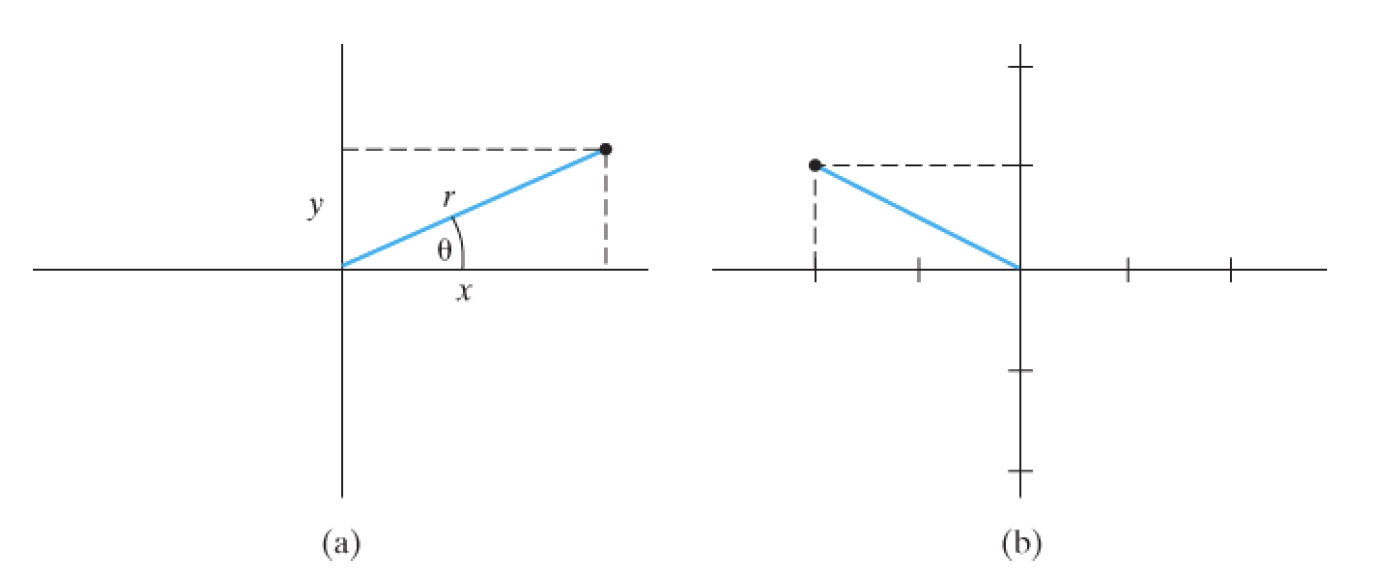
\includegraphics[width=0.8\textwidth]{/users/administrator/desktop/repo/quantumchemistry/Figures/1.3.png}  % 图片路径
		\caption{(a)\text{复数}$z = x + \mathrm{i}y$\text{的图象;}  (b)\text{复数}$-2+\mathrm{i}$\text{的图象}}
		\label{fig:1.3}
	\end{figure}\\
	\indent 如果$z$是实数,那么它的虚部为0。因此,当且仅当$z = z^{\ast}$时有$z$是实数。对复数$z$作两次复共轭,我们再次得到了$z$,所以$\left(z^{\ast}\right)^{\ast}=z$。将$z$与其复共轭$z^{\ast}$作乘积,我们有
	\begin{equation*}
		zz^{\ast} = \left(x + \mathrm{i}y\right)\left(x= \mathrm{i}y\right) = x^2+\mathrm{i}yx+\mathrm{i}xy-\mathrm{i}^2y^2
	\end{equation*}
	\begin{equation}
		\boxed{zz^{\ast} = x^2+y^2=r^2=\left|z\right|^2}
		\label{eq:1.30 product of z and its complex conjugate}
	\end{equation}
	对于两个复数$z_1=r_1\mathrm{e}^{\mathrm{i}\theta_1}$与$z_2 = r_2\mathrm{e}^{\mathrm{i}\theta_2}$的积和商,我们有
	\begin{equation}
		z_1z_2 = r_1r_2\mathrm{e}^{\mathrm{i}\left(\theta_1+\theta_2\right)}, \quad \frac{z_1}{z_2} = \frac{r_1}{r_2}\mathrm{e}^{\mathrm{i} \left(\theta_1 - \theta_2\right)}
		\label{eq:1.31 product and quotient of two complex numbers}
	\end{equation}
	\indent 根据复共轭的定义或 (\ref{eq:1.31 product and quotient of two complex numbers}),我们很容易证明
	\begin{equation}
		\boxed{\left(z_1z_2\right)^{\ast} = z_1^{\ast} z_2^{\ast}}
		\label{eq:1.32 properties of complex conjugate}
	\end{equation}
	同样地,
	\begin{equation}
		\boxed{
				\left(z_1/z_2\right) = z_1^{\ast} / z_2^{\ast}, \quad \left(z_1+z_2\right)^{\ast} = z_1^{\ast} + z_2^{\ast} , \quad \left(z_1-z_2\right)^{\ast} = z_1^{\ast} - z_2^{\ast}}
		\label{eq:1.33 linear properties of complex conjugate
		}
	\end{equation}
	对于积和商的绝对值,由(\ref{eq:1.31 product and quotient of two complex numbers})可知
	\begin{equation}
		\left|z_1z_2\right|=\left|z_1\right|\left|z_2\right|, \quad \left|\frac{z_1}{z_2}\right| = \frac{\left|z_1\right|}{\left|z_2\right|}
		\label{eq:1.34 properties of product and quotient absolute values}
	\end{equation}
	因此,如果$\psi$是复波函数,我们有
	\begin{equation}
		\left|\psi^2\right| = \left|\psi\right|^2 = \psi^{\ast} \psi
		\label{eq:1.35 properties of psi wave function}
	\end{equation}
	\indent 现在我们得到了数字 1 的 $n$ 次根式。我们可以将数字 1 的相位取为 0 或 $2\pi$ 或 $4\pi$,以此类推。因此 $1 = \mathrm{e}^{\mathrm{i}2\pi k}$,其中 $k$ 是任何整数,0、负数或正数。现在考虑数字 $\omega$,其中 $\omega \equiv \mathrm{e}^{\mathrm{i} 2\pi k /n}$,$n$ 为正整数。使用式(\ref{eq:1.31 product and quotient of two complex numbers}) $\:$$n$次,我们有$\omega^n = \mathrm{e}^{\mathrm{i}2\pi k} = 1$。因此,$\omega$是$n$次单位根。有 $n$ 个不同的复数 $n$ 次单位根,连续取 $n$ 个整数 $k$ 的值,就可以得到所有这些根:
	\begin{equation}
		\omega = \mathrm{e}^{\mathrm{i} 2\pi k /n}, \quad k = 0,1,2,\cdots , n-1
		\label{eq:1.36 n different complex nth roots of unity}
	\end{equation}
	除了 (\ref{eq:1.36 n different complex nth roots of unity}) 中的 $k$ 值之外,任何其他 $k$ 值所得到的数的相位都与 (\ref{eq:1.36 n different complex nth roots of unity}) 中的一个数相差 $2$ 的整数倍,因此不是不同的根。对于 (\ref{eq:1.36 n different complex nth roots of unity}) 中的 $n=2$,我们得到 1 的两个平方根;对于 $n=3$,得到 1 的三个立方根;以此类推。
	
	\section{单位}
	本书使用国际单位制。在国际单位制(SI)中,长度、质量、时间的单位分别是米(m)、千克(kg)和秒(s)。力的单位是牛顿(N),能量的单位是焦耳(J)。描述真空中相距 $r$ 的两个电荷 $Q_1$ 和 $Q_2$ 之间作用力大小的库仑定律,用国际单位制单位表示为
	\begin{equation}
		\boxed{F = \frac{Q_1Q_2}{4\pi \varepsilon_0r^2}}
		\label{eq:1.37 coulomb's law}
	\end{equation}
	其中电荷量$Q_1$和$Q_2$的单位是库伦(C),$\varepsilon_0$是常数(真空介电常数),其值为$8.854 \times 10^{-12} \mathrm{C}^2\mathrm{N}^{-1}\mathrm{m}^{-2}$。(物理常数的精确值见附录)
	
	\section{微积分学}
	量子化学中大量使用微积分,因此应牢记以下公式。其中 $c$、$n$ 和 $b$ 为常数,$f$ 和 $g$ 为 $x$ 的函数。
	\begin{equation*}
		\boxed{
			\frac{\mathrm{d}c}{\mathrm{d}x} = 0, \quad \frac{\mathrm{d}\left(cf\right)}{\mathrm{d}x} = c\frac{\mathrm{d}f}{\mathrm{d}x}, \quad \frac{\mathrm{d}x^n}{\mathrm{d}x} = nx^{n-1}, \quad \cfrac{\mathrm{d}\mathrm{e}^{cx}}{\mathrm{d}x} = c\mathrm{e}^{cx}
		}
	\end{equation*}
	\begin{equation*}
		\boxed{
			\frac{\mathrm{d}\left(\sin cx\right)}{\mathrm{d}x} = c \cos cx, \quad \frac{\mathrm{d} \left(\cos cx\right)}{\mathrm{d}x} = -c \sin cx, \quad \frac{\mathrm{d} \ln cx}{\mathrm{d} x } = \frac{1}{x}
		}
	\end{equation*}
	\begin{equation*}
		\boxed{
			\frac{\mathrm{d}\left(f+g\right)}{\mathrm{d}x} = \frac{\mathrm{d}f}{\mathrm{d}x}+\frac{\mathrm{d}g}{\mathrm{d}x}, \quad \frac{\mathrm{d}\left(fg\right)}{\mathrm{d}x} = f\frac{\mathrm{d}g}{\mathrm{d}x}+g\frac{\mathrm{d}f}{\mathrm{d}x}
		}
	\end{equation*}
	\begin{equation*}
		\boxed{
			\frac{\mathrm{d}\left(f/g\right)}{\mathrm{d}x} = \frac{\mathrm{d}\left(fg^{-1}\right)}{\mathrm{d}x} = -fg^{-2}\frac{\mathrm{d}g}{\mathrm{d}x}+g^{-1}\frac{\mathrm{d}f}{\mathrm{d}x}
		}
	\end{equation*}
	\begin{equation*}
		\boxed{
			\frac{\mathrm{d}}{\mathrm{d}x}f\left(g\left(x\right)\right) = \frac{\mathrm{d}f}{\mathrm{d}g}\frac{\mathrm{d}g}{\mathrm{d}x}
		}
	\end{equation*}
	最后一个公式有一个例子:$\mathrm{d}\left[\sin\left(cx^2\right)\right]/\mathrm{d}x = 2cx\cos\left(cx^2\right)$。这里$g\left(x\right) = cx^2$而$f=\sin$。
	\begin{equation*}
		\boxed{
			\int cf\left(x\right)\mathrm{d}x = c \int f\left(x\right)\mathrm{d}x, \quad \int \left[f\left(x\right)+g\left(x\right)\right]\mathrm{d}x = \int f\left(x\right)\mathrm{d}x+\int g\left(x\right)\mathrm{d}x
		}
	\end{equation*}
	\begin{equation*}
		\boxed{
			\int \mathrm{d}x = x, \quad \int x^n\mathrm{d}x = \frac{x^{n+1}}{n+1} \: \text{其中} \: n \neq -1, \quad \int \frac{1}{x}\mathrm{d}x = \ln x
		}
	\end{equation*}
	\begin{equation*}
		\boxed{
			\int \mathrm{e}^{cx}\mathrm{d}x = \frac{\mathrm{e}^{cx}}{c}, \quad \int \sin cx\mathrm{d}x = -\frac{\cos cx}{c}, \quad \int \cos cx\mathrm{d}x = \frac{\sin cx}{c}
		}
	\end{equation*}
	
	
	
	
	\section*{总结}

	\section*{习题}
